\textbf{See the instruction for questions \inteval{\value{question}+1} to \inteval{\value{question}+2}.}

\begin{figure}[H]
\centering
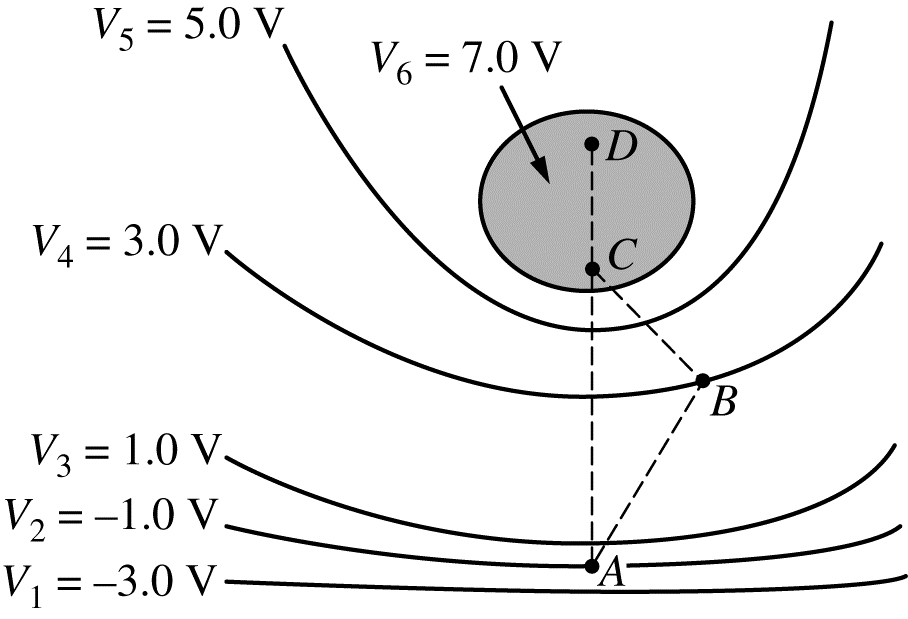
\includegraphics[scale=0.25]{images/img-013-039.png}
\end{figure}

Equipotential lines due to an electric field in a certain region of space are illustrated in the figure above. Points $A$ and $B$ are located on lines $V_{2}$ and $V_{4}$, respectively, and points $C$ and $D$ are located within the equipotential region $V_{6}$.

% Multiple Choice Question 30
\begin{questions}\setcounter{question}{29}\question
At which labeled point is the magnitude of the electric field the greatest?

\begin{oneparchoices}
\choice $A$
\choice $B$
\choice $C$
\choice $D$
\choice It is the same at all the points.
\end{oneparchoices}\end{questions}

% Multiple Choice Question 31
\begin{questions}\setcounter{question}{30}\question
How much work is required by an external force to move a $2.0 \unit{\mu C}$ charge from rest at point $A$ to rest at point $D$ via the path $ABCD$?

\begin{oneparchoices}
\choice $2.0 \unit{\mu J}$
\choice $3.0 \unit{\mu J}$
\choice $4.0 \unit{\mu J}$
\choice $12 \unit{\mu J}$
\choice $16 \unit{\mu J}$
\end{oneparchoices}\end{questions}

